\documentclass[10pt]{article}

\usepackage[margin=1in]{geometry}
\usepackage{amsmath, amssymb, amsthm}
\usepackage{booktabs}
\usepackage{graphicx}
\usepackage[hidelinks]{hyperref}
\usepackage{caption}

\newtheorem{lemma}{Lemma}

\title{Failure Modes of Belief-Propagation Decoding on\\
Degenerate Quantum LDPC Codes}
\author{Xiyuan Guo}
\date{\today}

\begin{document}
\maketitle

\begin{abstract}
This note quantifies \emph{why} belief propagation (BP) decoding fails
on degenerate quantum LDPC codes. Across exhaustive studies of small
codes and large-sample studies of surface-code patches and bivariate
bicycle codes, 98--100\% of the BP+OSD failures that an exact
minimum-weight decoder could have avoided are degenerate ambiguities
--- syndromes whose minimal errors span several logical classes ---
while classical stopping sets contribute zero. We calibrate the
fractional solutions of the Gu--Soleimanifar LP relaxation as a
detector of these ambiguities. A syndrome with two minimal errors
always places a fractional point in the optimal face of the LP, so the
detector reaches $100\%$ recall by construction, and its precision
decays with code distance from $48\%$ at $d \le 3$ to $9$--$21\%$ at
$d = 4$--$6$: degeneracy \emph{without} ambiguity is the sole source of
false positives. Finally, the [[144,12,12]] bivariate bicycle code
essentially never converges to a wrong answer, while [[72,12,6]] does
so on roughly $40\%$ of its BP failures.
\end{abstract}

\section{Introduction}

Belief propagation with ordered statistics decoding (BP+OSD) is the
default decoder for quantum LDPC codes, including the bivariate
bicycle codes of Bravyi et al.~\cite{bravyi2024}. It is known --- from
the SymBreak analysis of syndrome symmetry~\cite{symbreak} and from the
LP-decoding analysis of Gu and Soleimanifar~\cite{gusoleimanifar} ---
that \emph{degeneracy} is the root cause of BP's poor behavior on such
codes: a syndrome is degenerate when several minimal-weight error
patterns explain it, and decoding fails when those patterns disagree on
the logical outcome. What remains under-documented is the quantitative
split: how much of the avoidable failure is degenerate ambiguity versus
classical stopping sets versus plain non-convergence, and whether the
fractional solutions of the decoding LP relaxation predict those
failures.

This note provides that calibration. The contributions are:

\begin{itemize}
\item an exact minimum-weight decoding (MLD) oracle --- exhaustive
  enumeration for $n \le 13$ and integer programming (HiGHS MILP) for
  larger codes --- against which every decoder failure is classified as
  avoidable or not;
\item a small lemma: a syndrome with two minimal errors always carries
  a fractional point in the optimal face of the decoding LP, so
  face-fractionality detects \emph{all} ambiguous syndromes;
\item measured failure-mode tables for surface-code patches of distance
  $2$--$6$ and the [[72,12,6]], [[144,12,12]] bivariate bicycle codes,
  at four channel rates with fixed seeds.
\end{itemize}

\section{Setup and classifiers}

We work on the $X$-error side of CSS codes: a check matrix $h$ ($m
\times n$, over $\mathbb{F}_2$) detects bit-flip errors $e$, produces
the syndrome $s = h e$, and a logical matrix $\ell$ ($k \times n$) maps
an error to its logical class $\ell e$. The decoders are min-sum BP
with OSD post-processing (BP+OSD, combination sweep) and BP alone with
hard decisions; the MLD oracle enumerates, or solves by MILP, the
minimum-weight errors for a syndrome.

\begin{itemize}
\item \textbf{Avoidable failure.} A decode of error $e$ is an
  \emph{avoidable failure} when the MLD oracle decodes the same
  syndrome successfully but the decoder fails logically
  ($\ell(e \oplus c) \neq 0$).
\item \textbf{Degenerate ambiguity.} A syndrome is
  \emph{ambiguous} when its minimal errors carry more than one logical
  class. A failure is attributed to degenerate ambiguity when its
  syndrome is ambiguous.
\item \textbf{Stopping set.} A pattern is a stopping set when every
  check adjacent to its support touches at least two flipped positions.
  The test is applied to the true error support; on the residual it is
  vacuous for syndrome-valid corrections (every codeword support is
  trivially a stopping set).
\item \textbf{Convergence.} BP-only output satisfying all checks is a
  \emph{wrong convergence}; output violating the syndrome is a
  \emph{non-convergence}.
\end{itemize}

\section{An LP degeneracy detector}

Gu and Soleimanifar~\cite{gusoleimanifar} relax minimum-weight decoding
of a syndrome $s$ to a linear program over per-qubit indicators $x_i
\ge 0$ coupled to per-check, parity-consistent subset weights; the
objective $\sum_i x_i$ lower-bounds the minimal error weight. We call
an optimum \emph{fractional} when the \emph{optimal face} --- the set of
optima, not one solver vertex --- contains a point with a coordinate
strictly between $0$ and $1$. The face is characterized exactly: fix
the optimum value $v^\star$, then bound each coordinate's range on the
face with $2n$ additional LP solves.

\begin{lemma}
\label{lem:fractional}
Let $h$ be an $m \times n$ binary check matrix and $s$ a syndrome with
at least two distinct minimum-weight error patterns. Then the optimal
face of the Gu--Soleimanifar LP for $(h, s)$ contains a fractional
point.
\end{lemma}

\begin{proof}
Every error pattern $e$ is feasible with objective $\lvert e\rvert$:
for each check $j$ the subset $S_j = N(j) \cap \mathrm{supp}(e)$ has
parity $s_j$, so setting the corresponding subset weight to $1$
satisfies the parity and coupling constraints, giving $x = e$. Hence
$v^\star \le d_s$, the minimal error weight. If $v^\star < d_s$, no
integral feasible point attains $v^\star$ (an integral feasible point
is an error pattern of weight $v^\star$, contradicting minimality), so
every point of the face is fractional. If $v^\star = d_s$, two distinct
minimal errors $e_1 \neq e_2$ both lie on the face, and their midpoint
$(e_1 + e_2)/2$ is feasible by convexity with objective $d_s$ and
fractional coordinates wherever they differ.
\end{proof}

The lemma has two empirical consequences. First, every ambiguous
syndrome is detected: recall is $1$ \emph{by construction}, not by
luck. Second, the only false positives are multi-minimal-but-
unambiguous syndromes --- degeneracy without ambiguity --- which is
exactly the quantity this study measures. The single-solver-vertex
signal is strictly weaker: HiGHS returned integral vertices for most
degenerate syndromes, e.g.\ $0$ of the $2$ ambiguous syndromes of
[[5,1,2]].

\section{Experiments}

Two scales, all reproducible with fixed seeds:

\begin{itemize}
\item \textbf{Exhaustive} ($n \le 13$): every one of the $2^n$ error
  patterns is decoded and classified against the brute-force oracle;
  every rate is exact.
\item \textbf{Sampled} (Rivanna HPC): $10^4$ shots per rate for the
  distance $4$--$6$ surface patches (with the ILP oracle) and $10^5$
  shots per rate for the bicycle codes (decoder failure modes and LP
  calibration), at $p \in \{0.02, 0.05, 0.08, 0.10\}$.
\end{itemize}

The codes are the hypergraph product of two repetition codes
(surface-code patches) and qudec's bivariate bicycle constructions.
Table~\ref{tab:codes} summarizes the test set.

\begin{table}[ht]
\centering
\caption{Codes under test. Instances: patterns (exhaustive) or shots
per channel rate (sampled).}
\label{tab:codes}
\begin{tabular}{lcccccc}
\toprule
code & $[[n,k,d]]$ & $m$ & syndromes & instances & oracle & decoder \\
\midrule
Steane & $[[7,1,3]]$ & 3 & 8 & $2^7$ & brute force & BP / BP+OSD \\
rep5 & $[[5,1,5]]$ & 4 & 16 & $2^5$ & brute force & BP / BP+OSD \\
hgp22 & $[[5,1,2]]$ & 2 & 4 & $2^5$ & brute force & BP / BP+OSD \\
hgp32 & $[[8,1,2]]$ & 3 & 8 & $2^8$ & brute force & BP / BP+OSD \\
hgp33 & $[[13,1,3]]$ & 6 & 64 & $2^{13}$ & brute force & BP / BP+OSD \\
hgp44 & $[[25,1,4]]$ & 8 & -- & $10^4 \times 4$ & ILP & BP / BP+OSD \\
hgp55 & $[[41,1,5]]$ & 10 & -- & $10^4 \times 4$ & ILP & BP / BP+OSD \\
hgp66 & $[[61,1,6]]$ & 12 & -- & $10^4 \times 4$ & ILP & BP / BP+OSD \\
bb72 & $[[72,12,6]]$ & 36 & -- & $10^5 \times 4$ & none & BP / BP+OSD \\
bb144 & $[[144,12,12]]$ & 72 & -- & $10^5 \times 4$ & none & BP / BP+OSD \\
\bottomrule
\end{tabular}
\end{table}

\section{Results}

Table~\ref{tab:hgp} reports the failure-mode split for the degenerate
family at $p = 0.1$; Figure~\ref{fig:prec} shows the detector
calibration across distances, and Figure~\ref{fig:avoid} the avoidable
share of BP+OSD failures.

\begin{table}[ht]
\centering
\caption{Surface patches at $p = 0.1$. Rates over all patterns
(exhaustive rows) or $10^4$ seeded shots; ambiguity share of avoidable
BP+OSD failures; LP optimal-face precision/recall against avoidable
failures.}
\label{tab:hgp}
\begin{tabular}{lrrrrrrr}
\toprule
code & $P(\mathrm{fail})$ BP & $P(\mathrm{avoid})$ BP &
$P(\mathrm{fail})$ OSD & $P(\mathrm{avoid})$ OSD & ambig & prec & rec \\
\midrule
hgp22 & 0.1800 & 0.1476 & 0.1800 & 0.1476 & 1.000 & 0.500 & 1.000 \\
hgp32 & 0.2440 & 0.1978 & 0.2440 & 0.1978 & 1.000 & 0.494 & 1.000 \\
hgp33 & 0.1576 & 0.0869 & 0.1520 & 0.0803 & 1.000 & 0.403 & 1.000 \\
hgp44 & 0.183 & 0.130 & 0.149 & 0.088 & 1.000 & 0.214 & 1.000 \\
hgp55 & 0.211 & 0.155 & 0.139 & 0.069 & 0.996 & 0.091 & 1.000 \\
hgp66 & 0.246 & 0.196 & 0.143 & 0.072 & 0.996 & 0.091 & 1.000 \\
\bottomrule
\end{tabular}
\end{table}

\begin{figure}[ht]
\centering
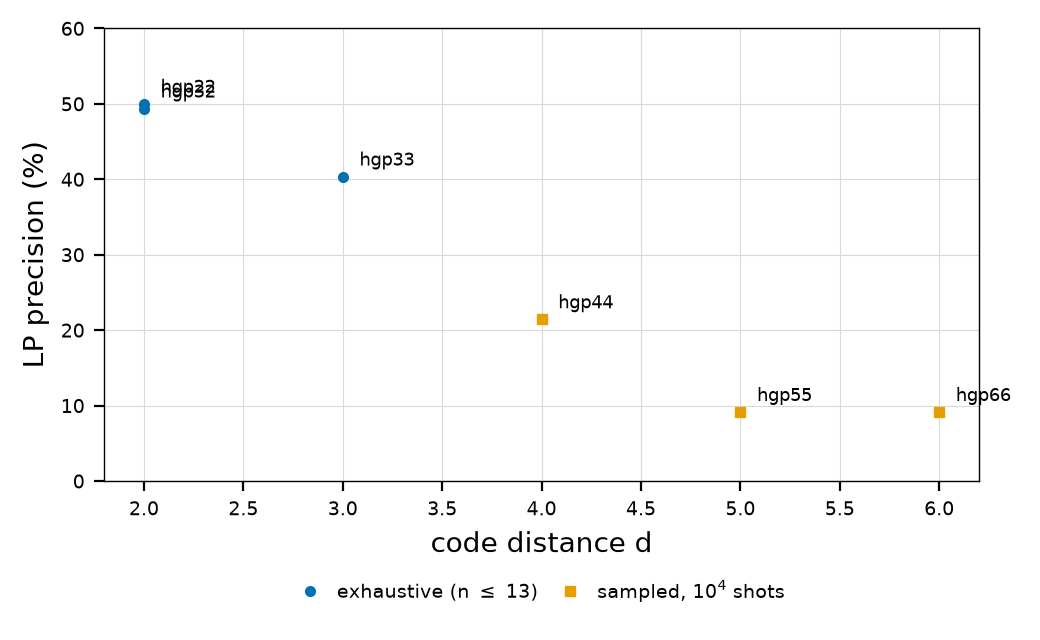
\includegraphics[width=0.78\textwidth]{figs/fig1_precision_distance.png}
\caption{Fractional-LP precision against avoidable BP+OSD failures
versus code distance, $p = 0.1$. Recall is $100\%$ at every point (by
Lemma~\ref{lem:fractional}). Precision decays as larger patches
accumulate degenerate-but-unambiguous syndromes.}
\label{fig:prec}
\end{figure}

\begin{figure}[ht]
\centering
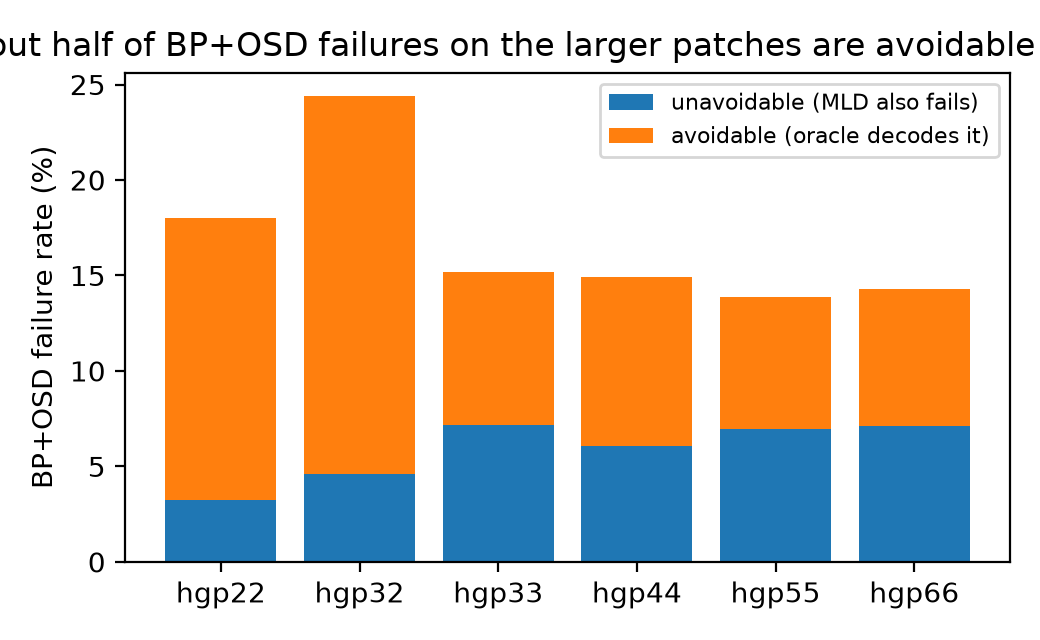
\includegraphics[width=0.78\textwidth]{figs/fig2_avoidable_share.png}
\caption{BP+OSD failure rate split into avoidable (the MLD oracle
decodes the same syndrome) and unavoidable, $p = 0.1$.}
\label{fig:avoid}
\end{figure}

\subsection{Finding 1: degeneracy, not stopping sets}

$98$--$100\%$ of avoidable BP+OSD failures are degenerate ambiguities
on every degenerate code at every rate (Table~\ref{tab:hgp});
stopping-set failures contribute zero everywhere. On the non-degenerate
controls the contrast is sharp: Steane has \emph{no} avoidable failures
at all (BP+OSD is MLD-optimal there), yet $3/8$ of its syndromes show
fractional LP faces --- the signal fires and flags nothing.

\subsection{Finding 2: the LP detector tracks degeneracy, not failure}

Recall is $100\%$ everywhere by Lemma~\ref{lem:fractional}; precision
decays with distance (Figure~\ref{fig:prec}) because large surface
patches accumulate multi-minimal-but-unambiguous syndromes. The vertex
signal would have missed most of this: $0$ fractional vertices on
[[5,1,2]] and [[8,1,2]], and $7$ of $33$ multi-minimal syndromes on
[[13,1,3]].

\subsection{Finding 3: roughly half of BP+OSD failures are avoidable}

At $p = 0.1$ the avoidable share of BP+OSD failures is $82\%$ on the
small patches and $50$--$59\%$ on the distance $4$--$6$ patches
(Figure~\ref{fig:avoid}); the remainder are true MLD limits. The
detector should therefore be read as a diagnosis tool for the
recoverable half, not as a failure predictor.

\subsection{Finding 4: the two bicycle codes fail differently}

Table~\ref{tab:bb} and Figure~\ref{fig:conv} show the decoder-side
calibration: on [[144,12,12]] only $3\%$ of BP failures are wrong
convergences (BP simply does not converge on the failures it makes),
while [[72,12,6]] wrong-converges on $37\%$ --- a clean
code-structure contrast. The LP precision against raw BP+OSD failures
rises with $p$ on both codes, from $0\%$ to $78\%$ on [[144,12,12]],
with recall $97$--$100\%$ wherever labeled syndromes exist.

\begin{table}[ht]
\centering
\caption{Bicycle codes, $10^5$ seeded shots per rate, no MLD oracle:
LP optimal-face precision/recall against BP+OSD failures, and the
wrong-convergence share of BP failures.}
\label{tab:bb}
\begin{tabular}{llrrrrr}
\toprule
code & $p$ & $P(\mathrm{fail})$ BP & $P(\mathrm{fail})$ OSD &
wrong-conv & prec & rec \\
\midrule
bb72 & 0.02 & 0.013 & 0.011 & 0.48 & 0.519 & 1.000 \\
bb72 & 0.05 & 0.180 & 0.160 & 0.47 & 0.679 & 0.935 \\
bb72 & 0.08 & 0.504 & 0.469 & 0.41 & 0.741 & 0.907 \\
bb72 & 0.10 & 0.699 & 0.663 & 0.37 & 0.858 & 0.897 \\
bb144 & 0.02 & 0.003 & 0.001 & 0.000 & 0.000 & n/a \\
bb144 & 0.05 & 0.103 & 0.052 & 0.037 & 0.188 & 1.000 \\
bb144 & 0.08 & 0.492 & 0.354 & 0.036 & 0.585 & 0.969 \\
bb144 & 0.10 & 0.758 & 0.635 & 0.033 & 0.776 & 1.000 \\
\bottomrule
\end{tabular}
\end{table}

\begin{figure}[ht]
\centering
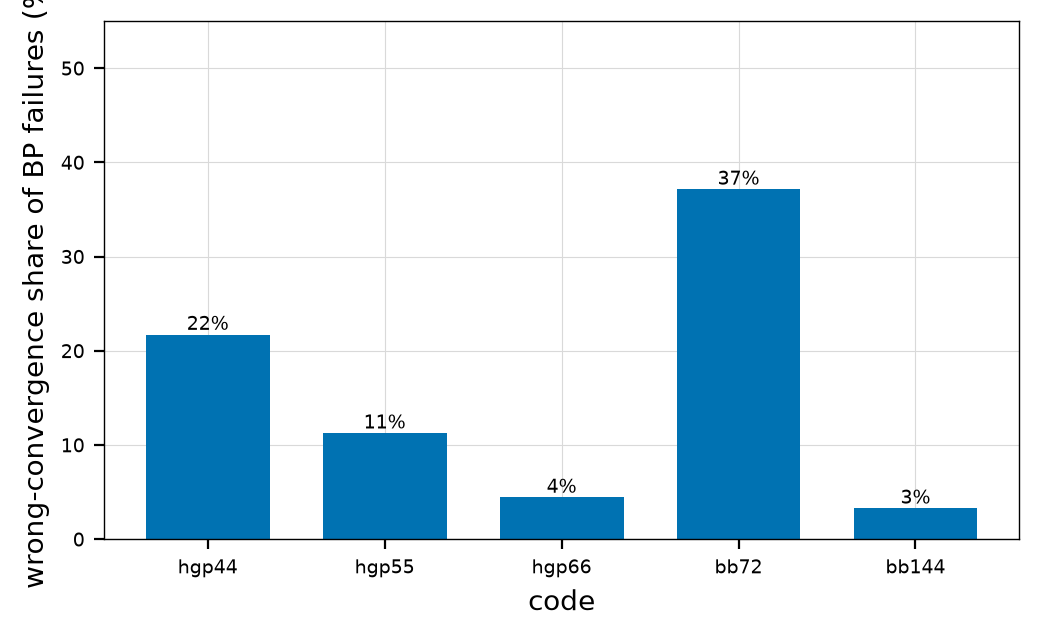
\includegraphics[width=0.78\textwidth]{figs/fig3_wrong_convergence.png}
\caption{Wrong-convergence share of BP failures at $p = 0.1$ across
the sampled codes (surface patches: avoidable failures; bicycle codes:
all failures).}
\label{fig:conv}
\end{figure}

\begin{figure}[ht]
\centering
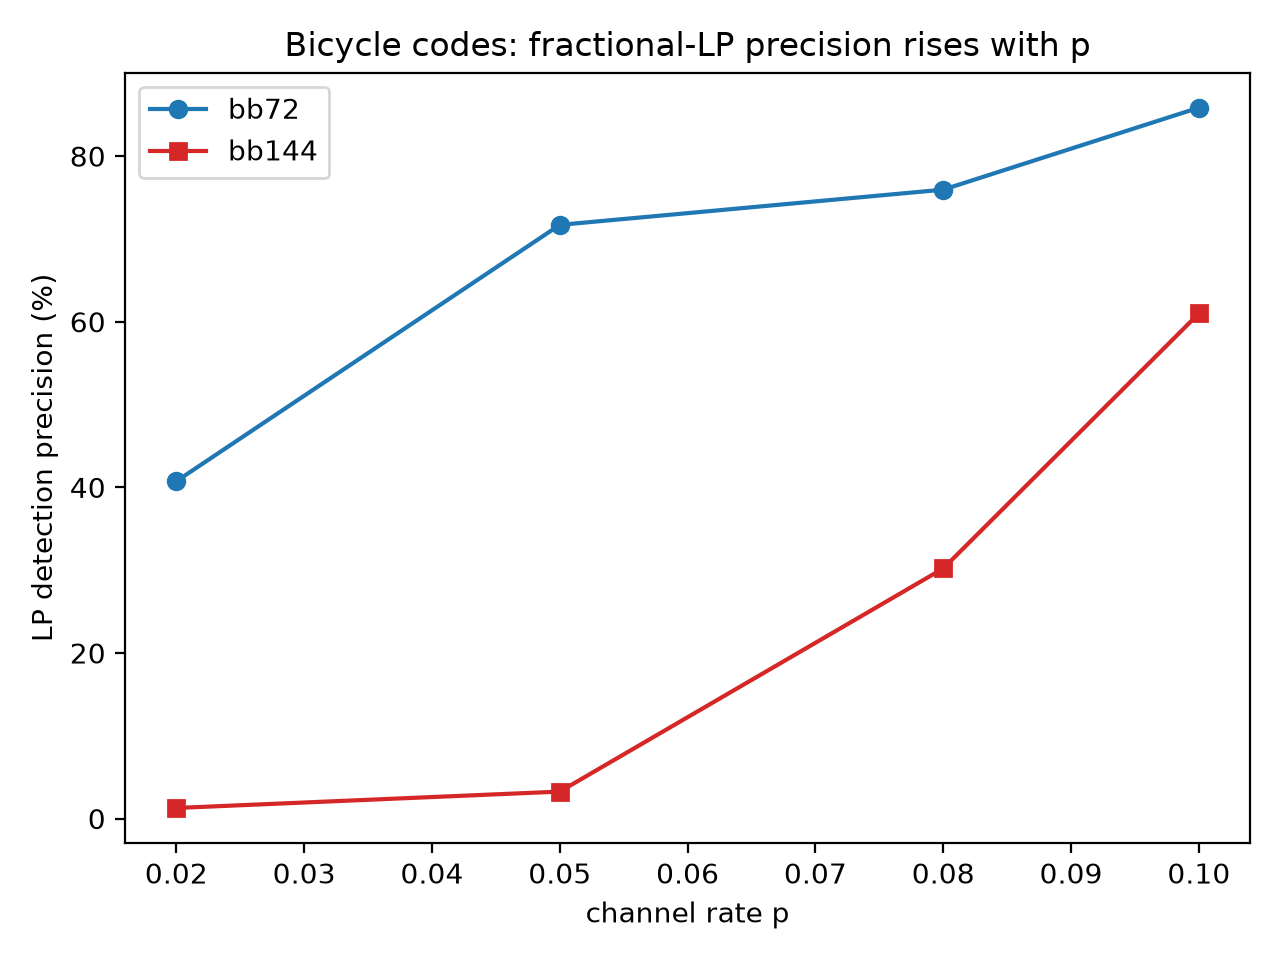
\includegraphics[width=0.7\textwidth]{figs/fig4_bb_precision.png}
\caption{Fractional-LP precision against BP+OSD failures versus $p$ on
the bicycle codes.}
\label{fig:bbprec}
\end{figure}

\section{Limitations and outlook}

\begin{itemize}
\item Code-capacity, $X$-error side only; one BP+OSD configuration
  (min-sum, 30 iterations, damping $0.9$, OSD-CS). The rates are single
  fixed-seed batches; multi-seed error bars are the obvious next step.
\item The LP face characterization costs $2n+1$ LP solves per
  syndrome, which caps the bicycle-code calibration at a few hundred
  sampled syndromes; the ILP oracle is exact but bounded by per-solve
  time limits (zero timeouts occurred here).
\item Ambiguity labels depend on the logical basis returned by the
  construction; the degenerate-family claims are robust to that choice.
\end{itemize}

\begin{thebibliography}{9}

\bibitem{bravyi2024}
S.~Bravyi, A.~W. Cross, J.~M. Gambetta, D.~Maslov, P.~Rall, and
T.~J. Yoder,
\newblock High-threshold and low-overhead fault-tolerant quantum
memory,
\newblock \emph{Nature} \textbf{627}, 778--782 (2024).

\bibitem{symbreak}
K.~Yin, X.~Fang, J.~Ruan, H.~Zhang, D.~Tullsen, A.~Sornborger,
C.~Liu, A.~Li, T.~Humble, and Y.~Ding,
\newblock SymBreak: Mitigating quantum degeneracy issues in QLDPC code
decoders by breaking symmetry,
\newblock arXiv:2412.02885 (2024).

\bibitem{gusoleimanifar}
S.~Gu and M.~Soleimanifar,
\newblock Power and limitations of linear programming decoder for
quantum LDPC codes,
\newblock \emph{IEEE Trans.\ Inf.\ Theory} \textbf{72}(10) (2026).

\bibitem{poulin2008}
D.~Poulin and Y.~Chung,
\newblock On the iterative decoding of sparse quantum codes,
\newblock \emph{Quantum Inf.\ Comput.} \textbf{8}(10), 987--1000
(2008).

\end{thebibliography}

\end{document}
